\section{Projeto eletrônico}

\subsection{Características Gerais}

Os sistemas eletrônicos que compõem o projeto são responsáveis por comandar os motores que despejam a ração na água de forma que a quantidade despejada e os períodos em que sejam despejados estejam de acordo com o que o usuário deseja. Ele também deve ser responsável por coletar dados importantes à piscicultura de forma que possam ser avaliados posteriormente. A seguinte figura ilustra como o sistema irá funcionar:

\begin{figure}[H]
 \centering
   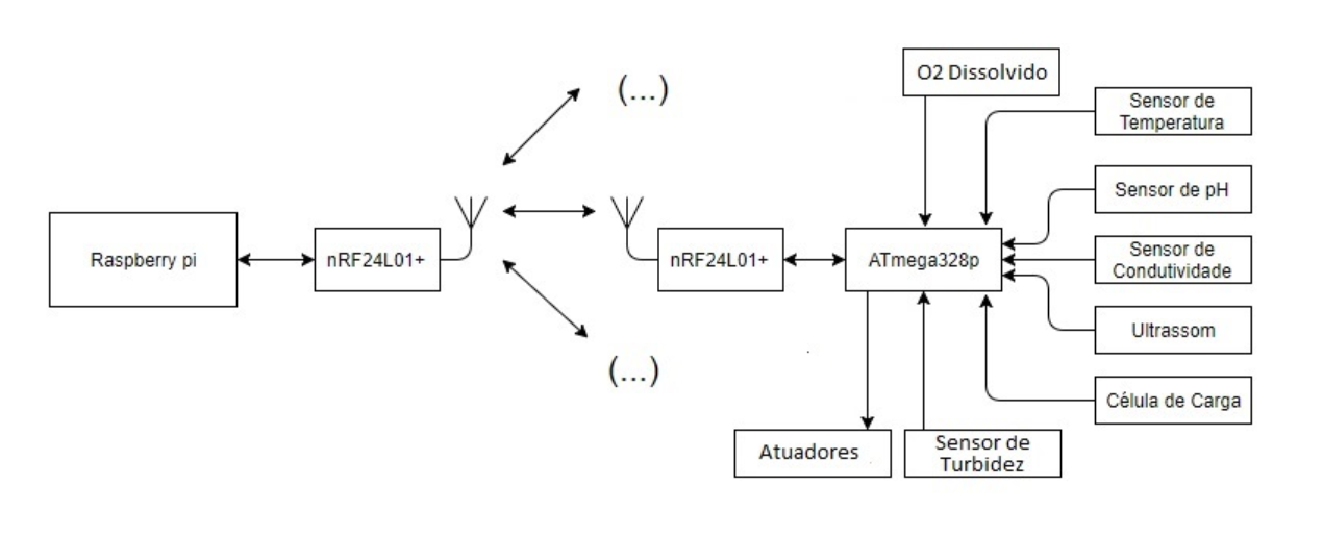
\includegraphics[keepaspectratio=true,scale=0.8]{figuras/componentes_eletronicos.eps}
 \caption{IIustração da organização dos sistemas eletrônicos.}
 \label{componentes}
\end{figure}

Uma Raspberry pi 3 B será o dispositivo central de comando que processará os dados e também funcionará como um servidor enviando informações para um servidor web. A Raspberry pi estará conectada a uma rede sem fio com os dispositivos presentes nas boias, que serão os dispositivos fim, por um módulo nRF24L01+ que enviará informações como o período em que as rações devem ser despejadas e a quantidade, e também receberá informações de sensoriamento realizado na boia. Os dispositivos eletrônicos nas bóias serão controlados por um microcontrolador ATmega328p que, conectado a um módulo nRF24L01+, também estará conectado à rede. O microcontrolador tem a  tarefa de receber as informações coletadas pelos sensores que avaliarão a temperatura, o pH, a condutividade da água, a sua turbidez e o O2 dissolvido nela, avaliarão também o nível de ração no primeiro compartimento e a porção de ração no segundo, ele também enviará os comandos para o controle do motor que rotaciona a rosca helicoidal que transporta a ração do primeiro para o segundo compartimento. Comanda também o motor que controla a abertura e fechamento do segundo compartimento para o despejo da ração. Os dados dos sensores serão enviadas pela rede para a central quando requisitados por ela. O microcontrolador também terá controle sobre o seu nível de bateria, indicando, quando requisitado pela central, este nível. A rede deverá suportar até 30 dispositivos finais. Os tópicos seguintes tratam sobre os dispositivos que compõem esta rede com mais detalhes.

\subsubsection{Sensores}
\subsubsubsection{Módulo Ultrassom}

\begin{figure}[H]
 \centering
   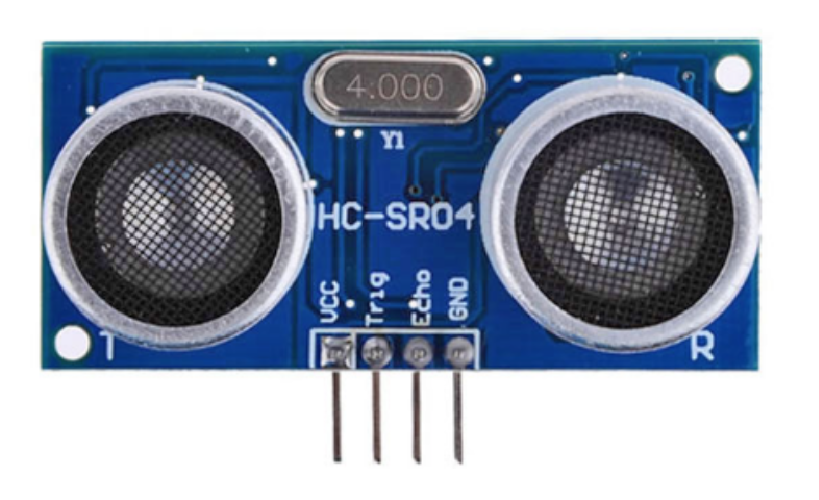
\includegraphics[keepaspectratio=true,scale=0.8]{figuras/ultrason.eps}
 \caption{Módulo HC-SR04}
 \label{ultrason}
\end{figure}

O módulo HC-SR04 é um dispositivo composto por um transmissor ultrassônico, sensor de ultrassom e um circuito de controle, este dispositivo pode medir uma distância de até 400cm com acurácia de 3mm. Este sensor será usado para medir o nível de ração no reservatório principal com o intuito de indicar, principalmente, quando ele deverá ser preenchido novamente. Algumas de suas especificações  mais importantes são:

\begin{itemize}
\item Tensão de alimentação DC: 5 V
\item Corrente de trabalho: 15mA
\item Frequência de trabalho 40 Hz
\item Máximo alcance: 4m
\item Mínimo alcance: 2cm
\item ângulo de medição: 15 graus
\end{itemize}

\subsubsubsection{Célula de Carga + Módulo condicionador de sinal}

\begin{figure}[H]
 \centering
   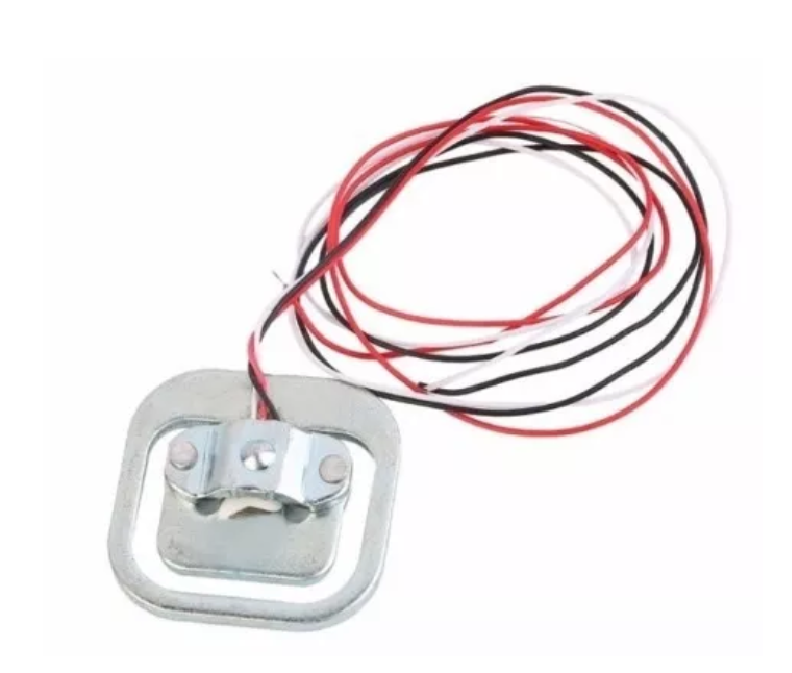
\includegraphics[keepaspectratio=true,scale=0.8]{figuras/celular_carga.eps}
 \caption{Célula de Carga}
 \label{celular_carga}
\end{figure}

\begin{figure}[H]
 \centering
   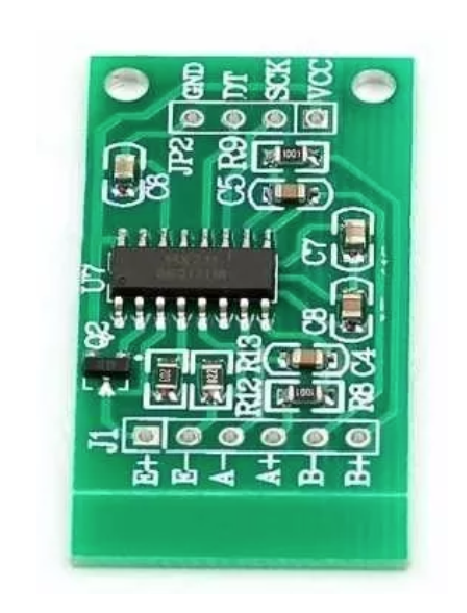
\includegraphics[keepaspectratio=true,scale=0.8]{figuras/modulo_h711.eps}
 \caption{Módulo Hx711}
 \label{modulo_h711}
\end{figure}

Para fazer a medição do peso da ração no segundo reservatório, com o intuito de controlar o quanto está sendo despejado de uma forma mais precisa, será utilizada uma célula de carga que suporta até 50kg. Quando a meia-ponte desta célula é esticada um sinal elétrico é enviado por um fio, este sinal analógico será tratado pelo módulo Hx711, um circuito de instrumentação que o converterá em um sinal digital de 24 bits, e enviado por uma interface I2C para o microcontrolador. As principais especificações dos dois componentes são:

Célula de Carga [12]:
\begin{itemize}
\item Capacidade de peso de cada cédula: Até 50kg
\item Potência nominal: 1,0 \underline{+} 0,1 mW
\item Impedância de entrada: 1000 \underline{+} 20% ohms
\item Impedância de saída: 1000 \underline{+} 10% ohms
\item Resistência de isolamento: 2000 ohms
\item Excitação Tensão: 5$V_{DC}$
\item Tensão máxima de trabalho: $8_{VCC}$
\item Material: Liga de Alumínio
\item Extensão dos fios: 10cm
\item Modo de conexão dos fios: Vermelho: sinal, Branco: terminal negativo, Preto: terminal positivo
\item Dimensões da Célula (CxLxA): 28 X 28 X 7mm
\item Dimensões do Case: 50 X 14,7mm
\item Peso: 25g
\end{itemize}

Hx711 [13]:
\begin{itemize}
\item 4,8V ~ 5,5V
\item Corrente de trabalho: 1,6mA
\item Conversor A/D com resolução de 24 bits
\item Canais A/D: 2
\item Dimensão: 2,9 x 1,7 x 0,4 cm (C x L x A)
\item Peso: 2 gramas
\end{itemize}

\subsubsubsection{Sensor de pH}

\begin{figure}[H]
 \centering
   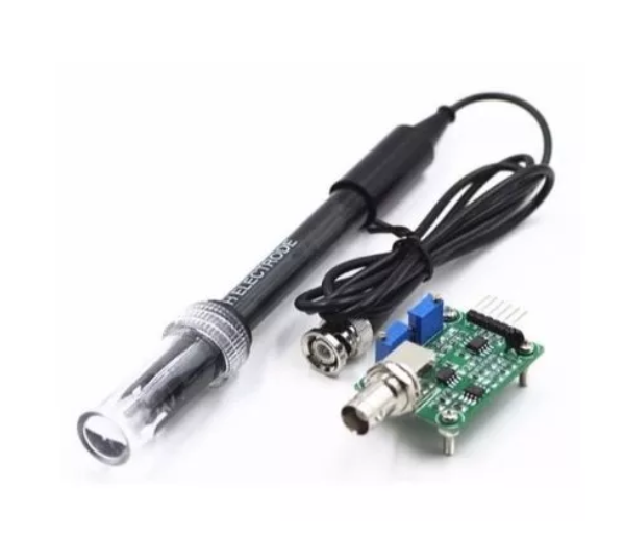
\includegraphics[keepaspectratio=true,scale=0.8]{figuras/sensorph.eps}
 \caption{Sensor de pH}
 \label{sensor_ph}
\end{figure}

O sensor de pH a ser usado é composto por um eletrodo de pH e um circuito de condicionamento de sinal analógico, os dois são unidos através de um conector BNC, o sinal fornecido ao final é analógico e deve ser conectado ao microcontrolador através de sua entrada analógica para posterior conversão ADC a ser realizada pelo microcontrolador. Especificações [14]:
\begin{itemize}
\item Tensão: 5 \underline{+} 0.2 V
\item Corrente de trabalho: 5-10mA
\item Potência: \underline{<} 0.5 W
\end{itemize}

\subsubsubsection{Sensor de Temperatura Ds18b20}

\begin{figure}[H]
 \centering
   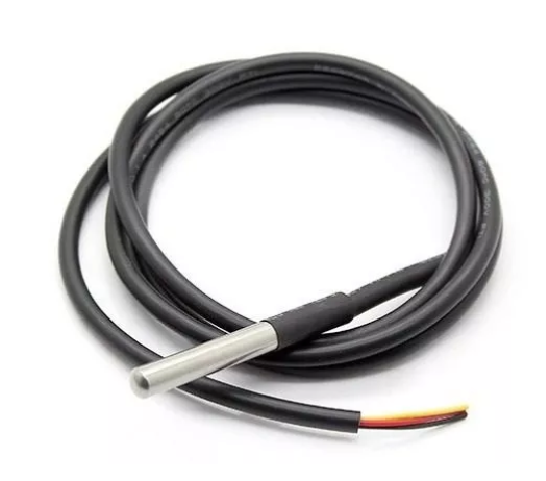
\includegraphics[keepaspectratio=true,scale=0.8]{figuras/sesortemperatura.eps}
 \caption{Sensor De Temperatura Ds18b20 à prova d’água.}
 \label{sensor_temperatura}
\end{figure}

Para a medição de temperatura será utilizado o sensor digital Ds18b20, ele é à prova d’água, possui resolução de medida de 9 a 12 bits, dependendo da configuração do usuário e comunicação 1-Wire com o microcontrolador. Algumas de suas especificações são:
\begin{itemize}
\item Tensão de alimentação: 3.0V ~ 5.5V
\item Corrente de trabalho: 1.5mA
\item Faixa de operação : -55{\degree}C  a +125{\degree}C  \underline{+} 0.5{\degree}C
\item Faixa de leitura: -10{\degree}C  a +85{\degree}C  \underline{+}0.5{\degree}C
\item Comprimento do cabo + conector: 1m
\end{itemize}

\subsubsubsection{Sensor de Condutividade}

\begin{figure}[H]
 \centering
   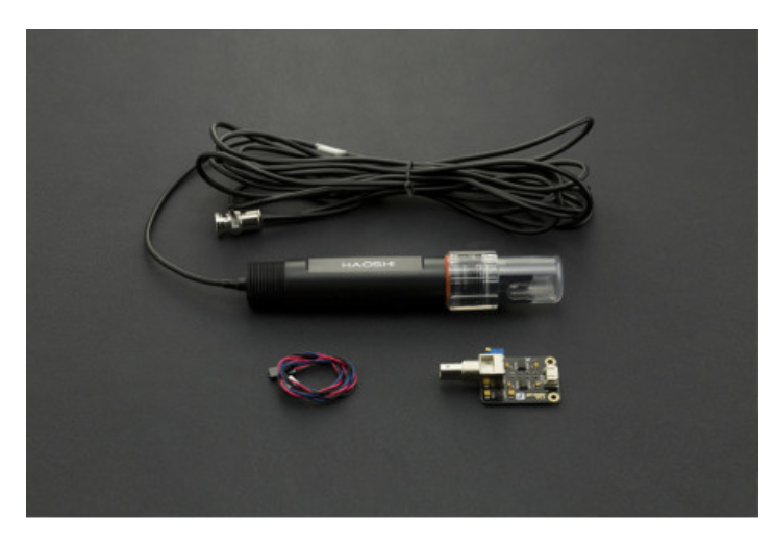
\includegraphics[keepaspectratio=true,scale=0.8]{figuras/sensorcodutividade.eps}
 \caption{Sensor de Condutividade}
 \label{sensor_condutividade}
\end{figure}

Para medir a condutividade foi escolhido utilizar o módulo DFR0300 juntamente com o eletrodo de conexão BNC para aplicações em medidas de EC (Electrical Conductivity), sua tensão de operação é de 5V com faixa de medição de 1ms/cm a 20ms/c, a comunicação com o microcontrolador é através de uma saída analógica.

\subsubsubsection{Sensor de O2 Dissolvido}

\begin{figure}[H]
 \centering
   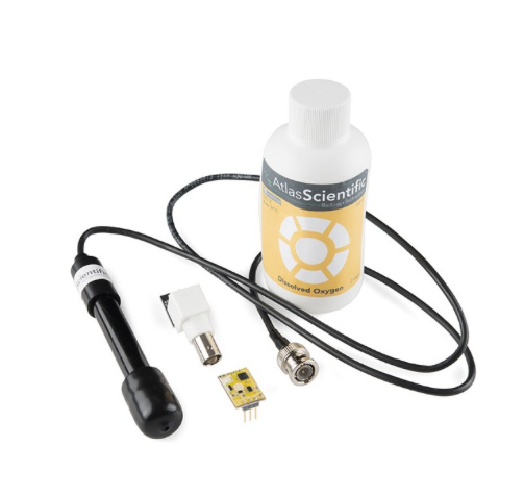
\includegraphics[keepaspectratio=true,scale=0.8]{figuras/sesoro2.eps}
 \caption{Sensor de O2 Dissolvido}
 \label{sensor_o2}
\end{figure}

Para a análise o oxigênio dissolvido será utilizado o módulo SEN-11194 que pode realizar a comunicação assíncrona através de uma porta UART, ou uma comunicação síncrona pelo protocolo I2C. Sua tensão de alimentação é de 5V com corrente máxima de 13.1mA.

\subsubsubsection{Sensor de Turbidez}

\begin{figure}[H]
 \centering
   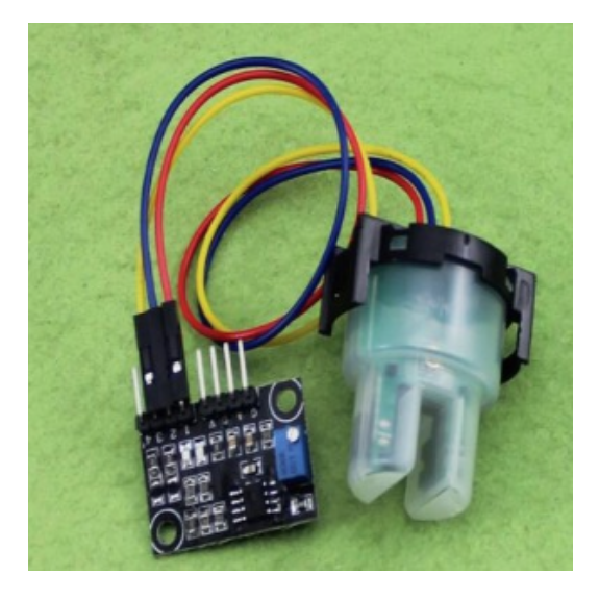
\includegraphics[keepaspectratio=true,scale=0.8]{figuras/sesortubidez.eps}
 \caption{Sensor de Turbidez}
 \label{sensor_tubidez}
\end{figure}

Para a medição de turbidez da água será utilizado o sensor LGZD Sensor V1.1 com saídas digitais (PWM) e analógicas. Trabalha com uma tensão de 5V e uma corrente máxima de 30mA.

\subsubsubsection{Monitoramento de Bateria}

Para evitar a desligamento do sistema devido a descarga da bateria e a consequente interrupção da alimentação dos peixes é necessário realizar o monitoramento do nível da bateria que alimenta o sistema. O monitoramento será feito por uma porta analógica, ele levará em conta duas características importantes da bateria: nível máximo quando estiver carregada, sendo considerado como 100\%, e o nível mínimo que ela pode chegar sem ser danificada, sendo considerado 0\%. Caso o valor da bateria seja maior do que o valor máximo de entrada da porta analógica então deve ser feito um circuito divisor de tensão, de acordo com a figura abaixo:

A equação \ref{divTensao} é usada para verificar quais serão os resistores que devem ser usados para construir o divisor.

\begin{figure}[H]
 \centering
   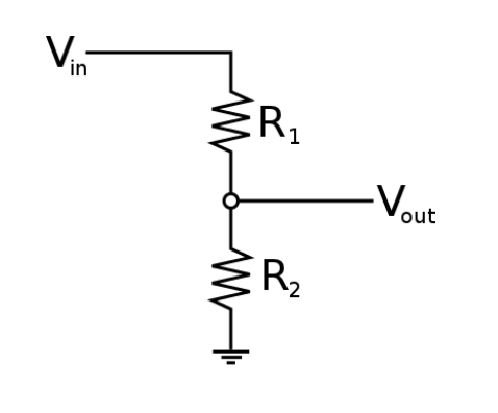
\includegraphics[keepaspectratio=true,scale=0.8]{figuras/divisortensao.eps}
 \caption{Divisor de Tensão}
 \label{divisor_tensao}
\end{figure}

\begin{equation}
\label{divTensao}
	V_{out}=V_{in}\frac{R_{2}}{R_{1}+R{2}}
\end{equation}
Onde $V_{in}$ é o nível máximo de tensão da bateria e $V_{out}$ o nível máximo que pode ser colocado na porta ADC [15]. É necessário também considerar a corrente máxima que o microcontrolador pode conduzir em sua porta GND, isto estabelece um valor mínimo para os resistores, sendo assim, de acordo com a lei de Ohm, e levando em consideração que a impedância de entrada da porta ADC é alta, a soma destes resistores é descrita na equação \ref{leiOhm}.
\begin{equation}
\label{leiOhm}
	R_{1}+R_{2}=\frac{V_{in}}{I}
\end{equation}
Sendo I a corrente que passa por eles.

\subsubsection{Atuadores}

\subsubsection{Comunicação}

A comunicação entre o dispositivo central, localizado em terra, e os dispositivos periféricos nas boias, em água, será feita através de uma rede sem fio, onde o dispositivo central envia informações de controle para os dispositivos periféricos, e também recebe dados destes dispositivos captados pelos sensores acoplados a eles. Para conectar os dispositivos a rede deve-se utilizar um módulo de comunicação sendo composto principalmente de um transceptor (dispositivo de envio e recepção de dados sem fio) que tenha baixo consumo de energia e baixa taxa de transferência de dados, considerando que as informações trocadas entre estes dispositivos são poucas. A comunicação será realizada a uma distância máxima de 200m, será então acoplada uma antena ao módulo de comunicação para aumentar a área de alcance do sinal. Levando estas informações em consideração será utilizado o seguinte dispositivo:

\subsubsubsection{Módulo nRF24L01+}

\begin{figure}[H]
 \centering
   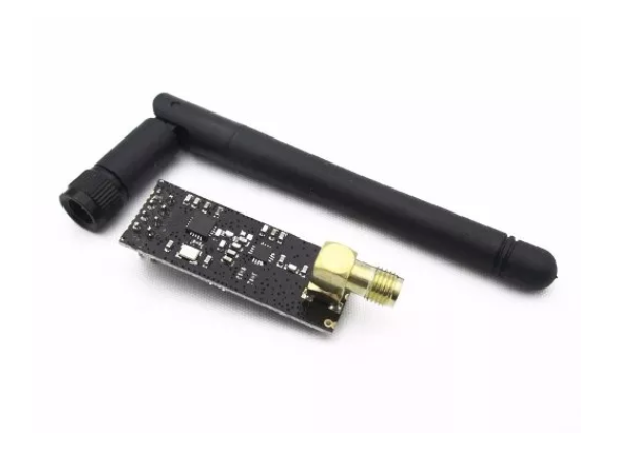
\includegraphics[keepaspectratio=true,scale=0.8]{figuras/modulonrf2.eps}
 \caption{Módulo nRF24L01+ com antenna omnidirecional.}
 \label{nRF24}
\end{figure}

Este módulo contém um chip transceptor de 2,4 GHz para uso em aplicações wireless de baixo consumo de potência, ele é configurado pelo microcontrolador ao qual ele está acoplado através de um protocolo Serial Peripheral Interface (SPI). O transceptor pode ser  configurado através de registradores acessados por SPI. Algumas características importantes deste módulo em conjunto com a antena são [4]:
\begin{itemize}
\item Tensão: 3.3V-3.6V (recomendado 3.3V)
\item Potência máxima de saída: 20 dBm
\item Consumo(transmitindo): 115mA(pico)
\item Consumo(recebendo): 45mA(pico)
\item Consumo(power-down): 4.2uA
\item Sensibilidade em modo de recepção 2Mbp:-92dBm
\item Sensibilidade em modo de recepção 1Mbps:-95dBm
\item Sensibilidade em modo de recepção 250kbps:-104dBm
\item Ganho do PA: 20dB
\item Ganho do LNA: 10dB
\item Figura de ruído do LNA: 2.6Db
\item Ganho da antena (pico): 2 dBi
\item Taxa de 2MB (área aberta): 520m
\item Taxa de 1MB (área aberta): 750m
\item Taxa de 250kb (área aberta): 1000m
\item Tamanho: 45,54 mm * 16,46 mm
\end{itemize}

\subsubsection{Controle e Processamento}

A aquisição de dados dos sensores, controle dos atuadores e processamento de dados serão feitos pelos seguintes sistemas:

\subsubsubsection{ATmega328p}

\begin{figure}[H]
 \centering
   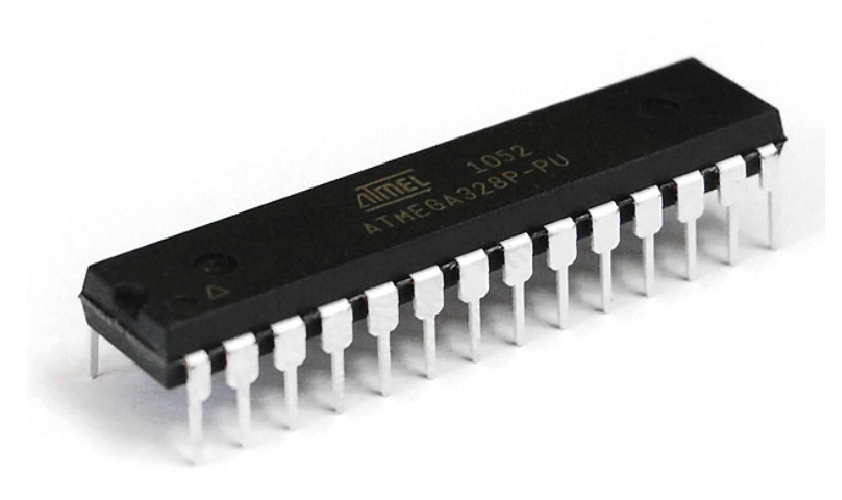
\includegraphics[keepaspectratio=true,scale=0.8]{figuras/atmega328.eps}
 \caption{ATmega328p}
 \label{ATmega328p}
\end{figure}

Para a aquisição dos dados dos sensores e controle dos atuadores presentes na boia será utilizado o microcontrolador ATmega328p, a recepção e envio de dados para o dispositivo central será feita através da conexão com o módulo nRF24L01+ descrito anteriormente. É um microcontrolador de baixo consumo de potência, de 8 bits e frequência máxima de operação de 20MHz, ele possui 6 canais ADC suficiente para o quantidade de sensores que serão utilizados. Algumas especificações importantes:

\begin{itemize}
\item Tensão máxima: 5.5V
\item Corrente máxima: 21.12mA
\item Entradas e saídas digitais: 23(6 PWM)
\item Entradas e saídas analógicas: 6
\item Memória Flash: 32 KB
\item Memória SRAM: 2KB
\item Memória EEPROM: 1KB
\end{itemize}

\subsubsubsection{Raspberry pi 3 B}

\begin{figure}[H]
 \centering
   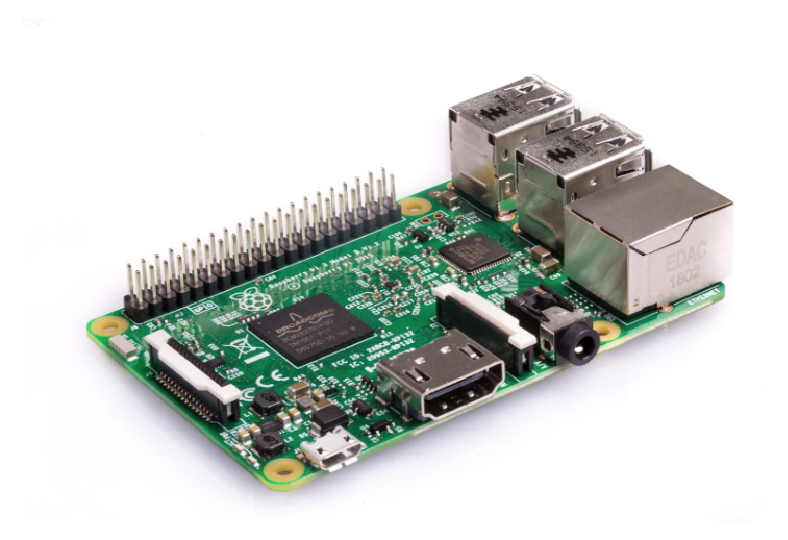
\includegraphics[keepaspectratio=true,scale=0.8]{figuras/raspberry.eps}
 \caption{Raspberry pi 3 B.}
 \label{Raspberry}
\end{figure}

O dispositivo central de processamento será constituído por uma Rapberry pi 3 B, ela será responsável por receber e enviar dados para os microcontroladores nas boias e também por processar dados e enviá-los para um servidor web através de seu módulo Wi-Fi. Algumas especificações importantes da placa são:
\begin{itemize}
\item Tensão de alimentação: 3.3V
\item Corrente: 50mA
\item SoC: Broadcom BCM2837
\item CPU: 4x ARM Cortex-A53, 1.2GHz
\item GPU: Broadcom VideoCore IV
\item RAM: 1GB LPDDR2 (900 MHz)
\item Rede: 10/100 Ethernet, 2.4GHz 802.11n wireless
\item Bluetooth: Bluetooth 4.1 Classic, Bluetooth Low Energy
\item Armazenamento: microSD
\item GPIO: 40-pin header, populated
\item Portas: HDMI, jack de audio-vídeo analógico de 3.5mm, 4x USB 2.0, Ethernet, Camera Serial Interface (CSI), Display Serial Interface (DSI)
\end{itemize}

\subsubsection{Projeto Energético}

\begin{table}[H]
\centering
\caption{Consumo elétrico total previsto dos componentes eletrônicos.}
\label{tabela_eletronica_energia}
\begin{tabular}{|l|l|}
\hline
Módulo ultrassom              & 75 mW   \\ \hline
Célula de carga               & 0,1 mW  \\ \hline
Módulo condicionador de sinal & 8 mW    \\ \hline
Sensor de temperatura         & 7,5 mW  \\ \hline
Sensor de condutividade       & 120mW   \\ \hline
Sensor de O2 dissolvido       & 65.5mW  \\ \hline
Sensor de turbidez            & 150mW   \\ \hline
Monitoramento de bateria      & 10mW    \\ \hline
Módulo wireless               & 400 mW  \\ \hline
Microcontrolador              & 100mW   \\ \hline
Total                         & 936.1mW \\ \hline
\end{tabular}
\end{table}

\subsubsection{Armazenamento}
\subsubsection{Recarga}
